\section{Local Optimizations}

Local Optimizations never goes away because this is always a piece of what happens even when we 
talk about even more sophiscated types of optimizations.

First we will talk about how to represent the code within a function or procedure, that's using 
something called a flow graph which is made of basic blocks.  Next we will contrast two different 
abstractions for doing local optimizations.




\subsection{Basic Blocks/Flow graphs} 


\subsubsection{Basic Blocks}

A basic block is a sequence of instructions(3-address statements). There are some requirements for basic 
block:

\begin{itemize}
    \item \textbf{Only the first instruction can be reached from outside the blcok.} The reason why this property 
    is useful is that within a basic block, we just march instruction by instruction through the block, 
    this simplies things at least within a basic block.
    \item \textbf{All the statements are executed consecutively if the first one is.}
    \item \textbf{The basic block must be maximal.} i.e., they cannot be made larger without violating conditions. 
\end{itemize}


\subsubsection{Flow graphs}
Flow graph is a graph representation of the procedure. In flow graph, basic blocks are the nodes, and the edge for \(  B_i 
\rightarrow B_j \) stands for a path from node \( B_i \) to node \( B_j \). So how will \(  B_i  \rightarrow B_j \) happen? 
There are two possibilities:

\begin{itemize}
    \item Either first instruction of \(B_j\) is the target of a goto at end of \(B_i\).
    \item \(B_j\) physically follows \(B_i\) which doesn't end in an unconditional goto.
\end{itemize}




% \begin{center}

% \begin{tikzpicture}[auto,
%     node distance = 12mm,
%     start chain = going below,
%     box/.style = {draw,rounded corners,blur shadow,fill=white,
%           on chain,align=center}]
%    \node[box] (b1)    {$x_1\leftarrow0$\\ $y_1\leftarrow0$};      
%    \node[box] (b2)    {$x_2\leftarrow\phi(x_1,x_3)$\\
%    $y_2\leftarrow\phi(y_1,y_3)$\\
%    $(x_2<10)$?};      
%    \node[box] (b3)    {$y_3\leftarrow y_2+x_2$\\ $x_3\leftarrow x_2+1$};  
%    \node[box] (b4)    {print($y_2$)};     
%    \begin{scope}[rounded corners,-latex]
%     \path (b2.-40) edge[bend left=50] (b4.40)
%     (b1) edge (b2) (b2) edge (b3);
%     \draw (b3.230) -- ++(0,-0.3) -| ([xshift=-5mm]b2.west) |-
%     ([yshift=3mm]b2.130) -- (b2.130);
%    \end{scope}
%   \end{tikzpicture}

% \end{center}




\subsubsection{Partitioning into Basic Blocks}

\begin{itemize}
\item Identify the leader of each basic block 
    \begin{itemize}
        \item First instruction
        \item Any target of a jump
        \item Any instruction immediately following a jump
    \end{itemize}

\item Basic block starts at leader and ends at instruction immediately before a leader(or the last instruction).    
\end{itemize}

An example of flow graph is shown below:

\begin{figure}[h]
    \centering
    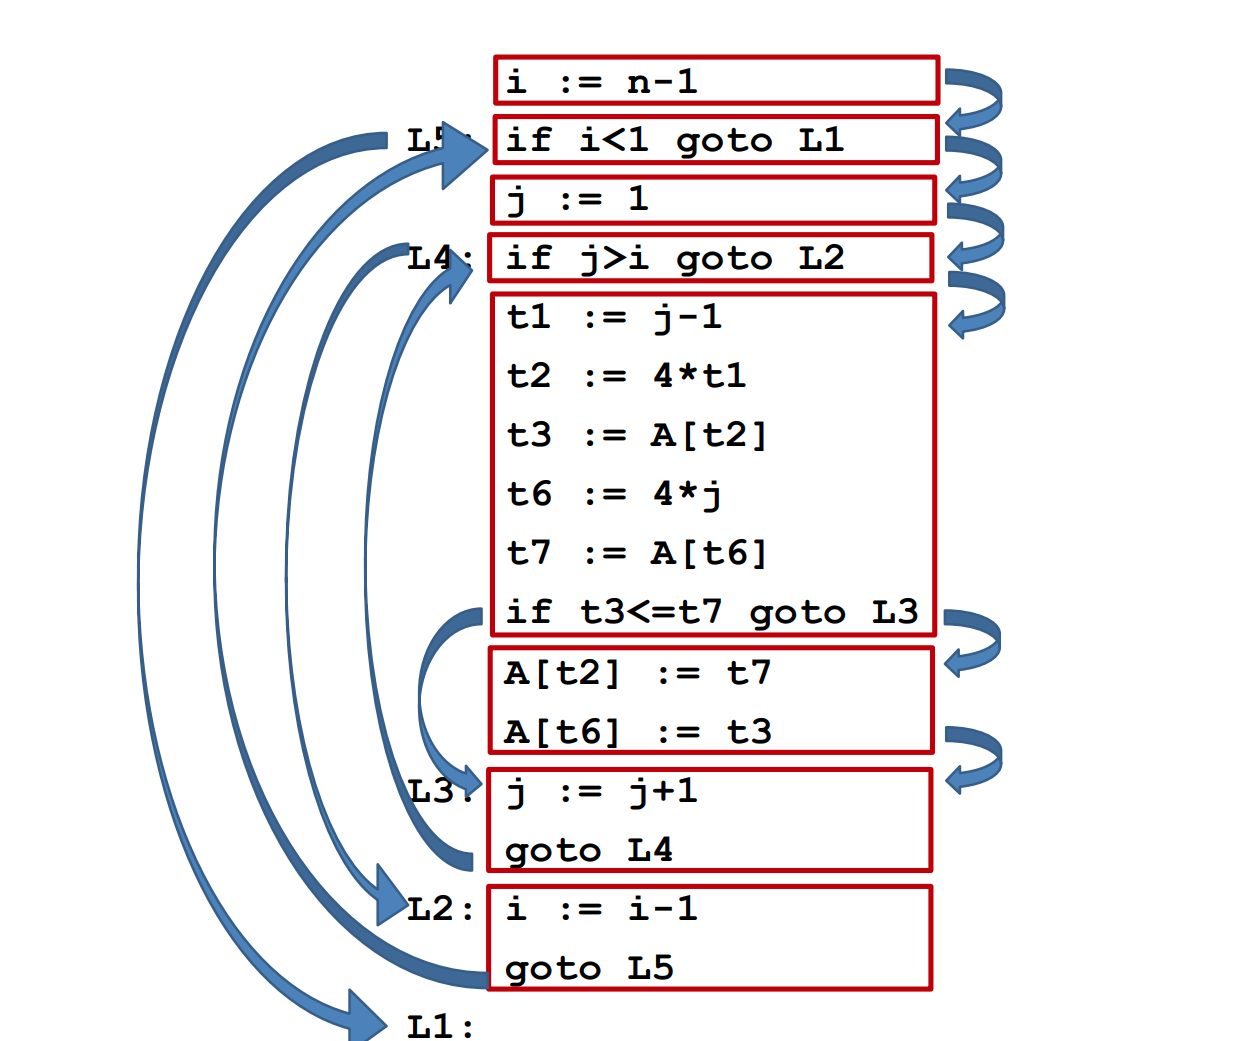
\includegraphics[width=0.5\textwidth]{flowgraph.png}
    \caption{Example of a flow graph}
\end{figure}

\subsubsection{Reachability of Basic Blocks}

There is one thing interesting need to mention here. So the source code is below:

\begin{lstlisting}[language=C, caption=An example]
if x { 
    ...
    return;
} else {
    ...
}


\end{lstlisting}


The corresponding flow graph is shown in \ref{fig:fgex}:

\begin{figure}[h]
    \centering
    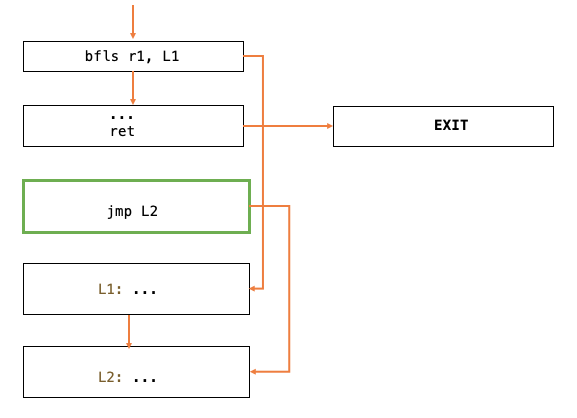
\includegraphics[width=0.5\textwidth]{fgex.png}
    \caption{Example of a flow graph}
    \label{fig:fgex}
\end{figure}


We can see that the box in green is unreachable from the entry. So why is that interesting? Typically, after compiers 
construct the control flow graph, they will go through and remove any unreachable nodes. Just do depth first traversal of the graph
from the entry node and mark all those visited nodes. So unmarked nodes will be deleted. This will help the compiler get a better optimization
result.


So why do these unreachable nodes appear? The anwser is it is not the job of the front-end of the compiler to clean up the unreachable nodes. 



\subsection{Local optimizations}

Local optimizations are those occur \textbf{within the basic blocks}. 
\subsection{Abtraction 1:DAG}


\subsection{Abtraction 2:Value numbering} 





